% -*- coding: utf-8 -*-
%-------------------------designed by zcf--------------
\documentclass[UTF8,a4paper,10pt]{ctexart}
\usepackage[left=3.17cm, right=3.17cm, top=2.74cm, bottom=2.74cm]{geometry}
\usepackage{amsmath}
\usepackage{graphicx,subfig}
\usepackage{float}
\usepackage{cite}
\usepackage{caption}
\usepackage{enumerate}
\usepackage{booktabs} %表格
\usepackage{multirow}
\newcommand{\tabincell}[2]{\begin{tabular}{@{}#1@{}}#2\end{tabular}}  %表格强制换行
%-------------------------字体设置--------------
% \usepackage{times} 
\usepackage{ctex}
\setCJKmainfont[ItalicFont=Noto Sans CJK SC Bold, BoldFont=Noto Serif CJK SC Black]{Noto Serif CJK SC}


\newcommand{\yihao}{\fontsize{26pt}{36pt}\selectfont}           % 一号, 1.4 倍行距
\newcommand{\erhao}{\fontsize{22pt}{28pt}\selectfont}          % 二号, 1.25倍行距
\newcommand{\xiaoer}{\fontsize{18pt}{18pt}\selectfont}          % 小二, 单倍行距
\newcommand{\sanhao}{\fontsize{16pt}{24pt}\selectfont}  %三号字
\newcommand{\xiaosan}{\fontsize{15pt}{22pt}\selectfont}        % 小三, 1.5倍行距
\newcommand{\sihao}{\fontsize{14pt}{21pt}\selectfont}            % 四号, 1.5 倍行距
\newcommand{\banxiaosi}{\fontsize{13pt}{19.5pt}\selectfont}    % 半小四, 1.5倍行距
\newcommand{\xiaosi}{\fontsize{12pt}{18pt}\selectfont}            % 小四, 1.5倍行距
\newcommand{\dawuhao}{\fontsize{11pt}{11pt}\selectfont}       % 大五号, 单倍行距
\newcommand{\wuhao}{\fontsize{10.5pt}{15.75pt}\selectfont}    % 五号, 单倍行距
%-------------------------章节名----------------
\usepackage{ctexcap} 
\CTEXsetup[name={,、},number={ \chinese{section}}]{section}
\CTEXsetup[name={(,)},number={\chinese{subsection}}]{subsection}
\CTEXsetup[name={,.},number={\arabic{subsubsection}}]{subsubsection}
%-------------------------页眉页脚--------------
\usepackage{fancyhdr}
\pagestyle{fancy}
\lhead{\kaishu \leftmark}
% \chead{}
\rhead{\kaishu 计算机网络实验报告}
\lfoot{}
\cfoot{\thepage}
\rfoot{}
\renewcommand{\headrulewidth}{0.1pt}  
\renewcommand{\footrulewidth}{0pt}%去掉横线
\newcommand{\HRule}{\rule{\linewidth}{0.5mm}}%标题横线
\newcommand{\HRulegrossa}{\rule{\linewidth}{1.2mm}}
%-----------------------伪代码------------------
\usepackage{algorithm}  
\usepackage{algorithmicx}  
\usepackage{algpseudocode}  
\floatname{algorithm}{Algorithm}  
\renewcommand{\algorithmicrequire}{\textbf{Input:}}  
\renewcommand{\algorithmicensure}{\textbf{Output:}} 
\usepackage{lipsum}  
\makeatletter
\newenvironment{breakablealgorithm}
  {% \begin{breakablealgorithm}
  \begin{center}
     \refstepcounter{algorithm}% New algorithm
     \hrule height.8pt depth0pt \kern2pt% \@fs@pre for \@fs@ruled
     \renewcommand{\caption}[2][\relax]{% Make a new \caption
      {\raggedright\textbf{\ALG@name~\thealgorithm} ##2\par}%
      \ifx\relax##1\relax % #1 is \relax
         \addcontentsline{loa}{algorithm}{\protect\numberline{\thealgorithm}##2}%
      \else % #1 is not \relax
         \addcontentsline{loa}{algorithm}{\protect\numberline{\thealgorithm}##1}%
      \fi
      \kern2pt\hrule\kern2pt
     }
  }{% \end{breakablealgorithm}
     \kern2pt\hrule\relax% \@fs@post for \@fs@ruled
  \end{center}
  }
\makeatother
%------------------------代码-------------------
\usepackage{xcolor} 
\usepackage{listings} 
\usepackage{graphicx}
\lstset{ 
breaklines,%自动换行
basicstyle=\small,
escapeinside=``,
keywordstyle=\color{ blue!70} \bfseries,
commentstyle=\color{red!50!green!50!blue!50},% 
stringstyle=\ttfamily,% 
extendedchars=false,% 
linewidth=\textwidth,% 
numbers=left,% 
numberstyle=\tiny \color{blue!50},% 
frame=trbl% 
rulesepcolor= \color{ red!20!green!20!blue!20} 
}
%------------超链接----------
\usepackage[colorlinks,linkcolor=black,anchorcolor=blue]{hyperref}
%------------------------TODO-------------------
\usepackage{enumitem,amssymb}
\newlist{todolist}{itemize}{2}
\setlist[todolist]{label=$\square$}
% for check symbol 
\usepackage{pifont}
\newcommand{\cmark}{\ding{51}}%
\newcommand{\xmark}{\ding{55}}%
\newcommand{\done}{\rlap{$\square$}{\raisebox{2pt}{\large\hspace{1pt}\cmark}}\hspace{-2.5pt}}
\newcommand{\wontfix}{\rlap{$\square$}{\large\hspace{1pt}\xmark}}
%------------------------水印-------------------
\usepackage{tikz}
\usepackage{xcolor}
\usepackage{eso-pic}
\usepackage{verbatim}

\newcommand{\watermark}[3]{\AddToShipoutPictureBG{
\parbox[b][\paperheight]{\paperwidth}{
\vfill%
\centering%
\tikz[remember picture, overlay]%
  \node [rotate = #1, scale = #2] at (current page.center)%
    {\textcolor{gray!80!cyan!30!magenta!30}{#3}};
\vfill}}}
\lstset{
  basicstyle=\ttfamily\small, % 使用打字机字体并设置为小号
  numbers=left,
}
%———————————————————————————————————————————正文
%----------------------------------------------
\begin{document}
\begin{titlepage}
    \begin{center}
    
\includegraphics[width=0.8\textwidth]{NKU.png}\\[1cm]    
    \textsc{\Huge \kaishu{\textbf{南\ \ \ \ \ \ 开\ \ \ \ \ \ 大\ \ \ \ \ \ 学}} }\\[0.9cm]
    \textsc{\huge \kaishu{\textbf{网\ \ 络\ \ 空\ \ 间\ \ 安\ \ 全\ \ 学\ \ 院}}}\\[0.9cm]
    \textsc{\huge \kaishu{\textbf{计算机网络实验报告}}}\\[0.8cm]
    \HRule \\[0.9cm]
    { \LARGE \bfseries Lab3-2 滑动窗口实现可靠传输}\\[0.4cm]
    \HRule \\[2.0cm]
    \centering
    \textsc{\LARGE \kaishu{2113946\ \ \ 刘国民 }}\\[0.5cm]
    \textsc{\LARGE \kaishu{年级\ :\ 2021级}}\\[0.5cm]
    \textsc{\LARGE \kaishu{专业\ :\ 信息安全}}\\[0.5cm]
    \vfill
    {\Large \today}
    \end{center}
\end{titlepage}



\newpage
\tableofcontents
\setcounter{page}{1}

\vspace{1cm}

\section{实验内容}
本次实验在实验3-1的基础上,引入基于滑动窗口的流量控制机制,采用累积确认的方式,完成给定测试文件的传输。同时在传输完成后,会计算传输时间和吞吐率等相关性能指标,并改变路由程序的丢包率和延时来进行分析。
\vspace{1cm}

\section{协议设计}
协议设计分为报文格式、差错检验、建立连接、数据传输和关闭连接五个部分。该部分重点阐述本次实验不同于上次实验的地方(即数据传输部分),差错检验、报文格式、三次握手以及四次挥手的协议设计与上次实验基本一致,本次实验只作简要叙述、
\subsection{报文格式}
本次实验中采用以下结构的数据报:
\begin{lstlisting}[frame=trbl,language={C++}]
struct Datagram {
    bool ack, syn, fin;
    uint16_t checksum;//16位校验和
    long long seqnum, acknum;
    int DataLen;// DataLen<=MaxBufferSize
    char data[MaxBufferSize] = { 0 };
}SendData, ReceiveData;
\end{lstlisting}\par
与上次实验一样,依旧用结构体将原始发送数据与ack,syn,fin等标志位和校验和等协议开销封装在一起。SendData,ReceiveData用来填充每次发送和接收的数据包\par


\subsection{差错检验}
差错检验使用以下算法实现:
\begin{enumerate}
    \item 将数据报按16bit为一组进行分组,不足一组的用0补齐
    \item 将checksum字段置0
    \item 按位累加所有组的值,每次相加如果最高位有溢出则补到16位数的最低位上
    \item 将上述步骤的结果取反后填入checksum字段
\end{enumerate}\par
需要注意的是,实验中用RECEIVE\_CHECK和SEND\_CHECK两个宏来标识是否取反,发送的时候需要取反,接受时则不用取反,接收时验证算出的校验和与数据包的校验和字段相加是否为0xffff即可。

\subsection{建立连接}
依旧采用以下方式建立连接:
\begin{enumerate}
    \item 首先发送方发送一个空数据报给接收方(全为0),仅将syn标志位置为1,表示发送方请求建立连接。同时阻塞等待接收方的syn+ack包。
    \item 接收方持续阻塞等待发送方的syn包,如果成功接收到syn标志位为1的数据包,则将一个空包的syn、ack和acknum位置为1后发回,告诉发送方成功收到seqnum为0的syn包。
    \item 发送方成功收到syn+ack包后,发回一个ack包,同时设置seqnum和acknum为1,表示成功收到seqnum为0的syn+ack包,同时序列号自增1。至此连接建立完成,
\end{enumerate}\par
建立连接的具体流程基本与TCP三次握手一致,在这里双方的初始序列号ISN均取0。

\subsection{传输数据}
本次实验设计的协议类似于GBN协议,但不同于GBN协议的是,协议中使用的是非重复序列号,即从0号包开始,不使用循环序列号。接收端持续跟踪期望的序列号即可、下面重点阐述是如何传输数据的。
\subsubsection{滑动窗口机制}
本次实验与实验3-1最大的不同在于,允许发送方在没有接收到确认(ACK)的情况下发送多个数据包,而不需要发送一个数据包等一个ACK回复然后再开始发送下一个。详细说明如下:
\begin{itemize}
\item 窗口大小:窗口大小即传输前预先设定的一个数值,表示发送方在等待ACK之前可以发送的最大数据包数量。在未到达窗口右边界之前,发送端将不断发送数据包给接收端。
\item 累积确认:接收端发回的ACK代表在此之前的数据包全部收到。同时接收端维护一个期望序列号的变量,如果收到数据包的序号大于期望值,则丢弃数据包并发回一个期望值-1的ACK;如果收到数据包序号等于期望值,则发回一个期望值序号的ACK,同时期望值+1;如果收到数据包的序号小于期望值则直接丢弃即可,但也需要发回一个期望值-1的ACK。
\item 窗口右移:发送方用一个变量Base来记录窗口的左边界,只有当收到acknum大于或等于Base时,窗口才向右移动。可以知道,acknum的含义是接收端已经收到在此之前的数据包,所以不管acknum大于还是等于Base,窗口右移时移动到acknum+1即可,即Base=acknum+1。同时,由于窗口左边界的移动,右边界也会相应向右移动,进而发送新的数据包给接收端。
\item 超时重传:发送端在发出Base包或者右移到新的窗口值时,会启动定时器来等待接收端的ACK,如果超过设置的时间后,需要将整个窗口重传一次,并重新为Base包开启定时器。
\item 流量控制:通过限制在确认之前可以发送的数据包数量来实现流量控制。这也是设置窗口大小的意义所在。
\end{itemize}\par
基于上述协议,整体的传输流程即是:发送端不断发送数据包,到达发送上限,等待ACK回复,收到正确回复就右移窗口继续发送,超时即重传整个窗口;接收端持续接收数据包,不是需要的数据包序号则丢弃。窗口图示如下:
\begin{figure}[H]
    \centering
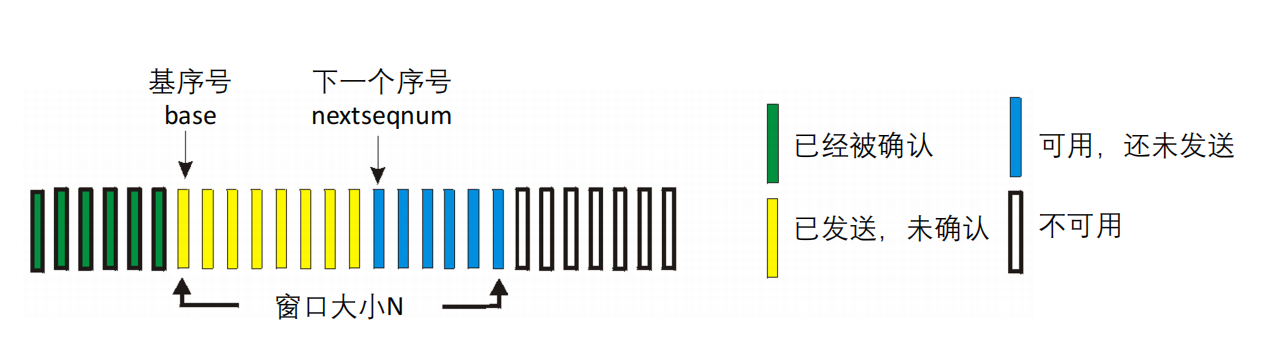
\includegraphics[width=0.6\textwidth]{img/滑动窗口.png}
    \caption{滑动窗口}
\end{figure}

\subsubsection{情形分析}
基于设计的协议,我们分析丢失、错误等情形下该协议是怎么运转的。
\begin{enumerate}
    \item 发送数据包丢失/出错: 发送端的数据包丢失后,在此之前的数据包都能收到正确的ACK回复,窗口左边界滑动到该包时,发送端开启定时器,接收端也在一直等待该包或者出错时丢弃,发送端无法收到ACK回复,超时后将该包之后的数据包全部重传。
    \item ACK/丢失/出错/提前超时:假设发送端发送一个Base=x的数据包,为它开启定时器,接收端正确收到数据包但回复丢失、出错或超时。在此情况下发送端重发整个窗口,由于上次已经成功接收,此时接收端期望的序列号已经是x+1,但收到的数据包序号小于期望值时,也会发回acknum=x的回复,而发送端收到acknum=Base的回复,直接移动窗口即可,传输继续正常进行。
\end{enumerate}

\subsection{关闭连接}
关闭连接也使用与TCP协议类似的流程,如下图所示:
\begin{figure}[H]
    \centering
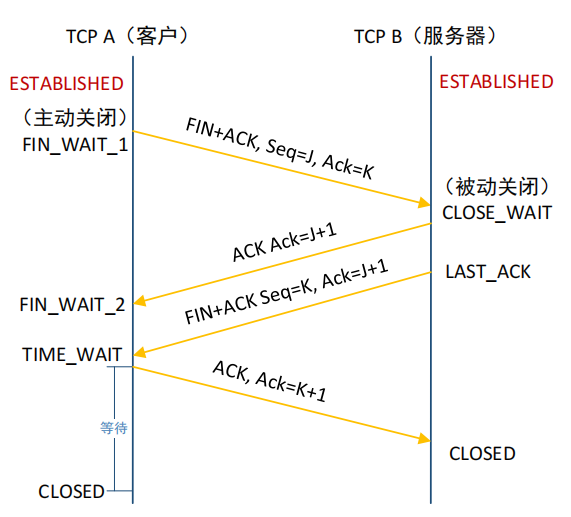
\includegraphics[width=0.6\textwidth]{img/关闭连接.png}
    \caption{关闭连接}
\end{figure}
如上图所示,但序列号J和K在此处跟三次握手类似,均取为0。

\section{代码实现}
代码实现部分主要分析传输数据部分的代码,差错检验、Socket初始化、建立和关闭连接的代码与上次实验相同,不再赘述。建立连接时,我将文件名放入了第三次握手ACK报文的空闲缓冲区,一起发送给接收端。
\subsection{发送端}
根据协议设计,发送端的总体实现思路如下:
\begin{itemize}
\item 发送端用主线程main和两个创建的子线程Resend和Timer完成协议给出的功能和操作。
\item 主线程main负责发送数据包,即一旦窗口左边界右移,主线程负责发送新的数据包给接收端。
\item 子线程Resend负责持续检测是否“超时”,“超时”则重传,这里的“超时”指的是在指定时间内没有收到正确的acknum(即acknum>=Base)
\item 子线程Timer负责为Base包开启定时器,一旦超时则通知线程Resend,这里的“通知”是通过全局变量的设置来实现,稍后会在具体的代码实现中看到。
\end{itemize}
首先我们给出下列全局变量:
\begin{lstlisting}[frame=trbl,language={C++}]
// 多线程共享数据,写数据的时候用互斥锁
int Flag_Resend = 0;// 表示recvfrom的数据是否超时
int Flag_Timer = 0;// 表示是否需要启用定时器服务
int SeqNumber = 0;// 记录一共有多少个数据包,seqnum:0--SeqNumber-1
long long Base = 0;// 初始序列号从0开始
long long NextSeq = 0;
\end{lstlisting}\par
从注释中可以看到,Flag\_Resend用于表示收到的数据是否超时,只要子线程Timer发现超时了就将该标志位置为1,这时候子线程Resend就可以检测到,从而开始重发窗口中的数据包。Flag\_Timer用于表示是否需要开启定时器,即主线程或者Resend线程发送Base包,或者窗口右移更新Base值的时候,就将该标志位置为1,Timer线程就会开始启用定时器,持续接收可能的ACK回复。而Base,NextSeq和SeqNumber为全局变量,为三个线程共同使用。\par
在本次实验中,我们用一个vecotr容器来保存所有要传输的数据包,在传输之前我们先把原始文件以4096字节为一组放入vector中,具体代码如下:
\begin{lstlisting}[frame=trbl,language={C++}]
// 移动文件指针到文件末尾
fseek(p, 0, SEEK_END);
long long FileLen = ftell(p);
fseek(p, 0, SEEK_SET);
long long temp = FileLen;
// 数据以4096字节为单位放入vector序列
while (temp>0) {
    SendData = { 0 };
    fread(SendData.data, MaxBufferSize, 1, p);
    SendData.DataLen = temp < MaxBufferSize ? temp : MaxBufferSize;
    SendData.seqnum = SeqNumber++;
    v.push_back(SendData);
    temp -= SendData.DataLen;
}
\end{lstlisting}\par
fread将数据读取到发送数据包缓冲区中,将相关信息封装好后放入容器,之后涉及重传的时候,直接从容器中拿取数据包重发即可,对于窗口的滑动,直接增加Base,NextSeq等变量后通过vector随机访问即可,SeqNumber用来记录一共有多少个数据包。接下来我们逐个分析三个线程的具体代码。
\begin{lstlisting}[frame=trbl,language={C++}]
while (true) {
    if (NextSeq == SeqNumber) {// 发送完毕
        break;
    }
    if (NextSeq < Base + WindowSize) {
        SendData = v[NextSeq];
        Send();
        if (NextSeq == Base) {// 第一个包
            lock_guard<mutex> lock(mtx);
            Flag_Timer = 1;
        }
        {
            lock_guard<mutex> lock(mtx);
            NextSeq++;
        }
        Sleep(100);;//每次发送睡眠100毫秒,避免短时间内发送大量数据包给接收方
    }
}
\end{lstlisting}\par
上述代码是main函数中发送数据的核心代码,整体逻辑是持续检测NextSeq是否小于Base+WindowSize,即发送的数据包是否到达右边界,如果没到达就持续发送并增加NextSeq的值。如果发送的是Base包则需要设置Timer标志位,通知子线程启动定时器。其中v即是上述提到的vector容器,需要注意在这个过程中,对多线程的共享数据(这里为Flag\_Timer)进行写操作时,需要使用互斥锁以阻塞子线程进行操作,避免多线程同时进行写操作从而引发错误。每次发送后,使用sleep函数睡眠100毫秒,避免短时间发送大量数据包给接收方。如果NextSeq如果等于SeqNumber,则代表窗口右边界已经到达容器末尾,此时主线程直接break退出循环即可。后续可能涉及到的重传由Resend完成。
\begin{lstlisting}[frame=trbl,language={C++}]
void Resend() {// 只要检测到Flag_Resend变为1就重发Base--(NextSeq-1)
    while (true) {
        if (Flag_Resend == 1) {
            BackCounter++;
            for (int i = Base; i <= NextSeq-1; i++) {
                SendData = v[i];
                Send();
                if (i == Base) {//Base包
                    lock_guard<mutex> lock(mtx);
                    Flag_Timer = 1;//启动定时,通知Receive线程
                }
            }
            {
                lock_guard<mutex> lock(mtx);
                Flag_Resend = 0;
            }
        }
        if (Base==SeqNumber) {//传输完毕
            cout << "[提示]:ReSend线程正确结束" << endl;
            return;// 结束进程
        }
    }
}
\end{lstlisting}\par
上述代码是子线程Resend绑定的函数,核心逻辑就是while循环持续检测Flag标志位,如果为1就开始重传窗口,重传数据也是通过容器v获得,BackCounter用于记录整个传输过程中的重传次数。与主线程类似,发送Base包需要启动定时器,写操作使用互斥锁。当Base=SeqNumber,即左边界也到达文件末尾时,此时退出循环。
\begin{lstlisting}[frame=trbl,language={C++}]
void Timer() {// 持续监测Flag_Timer,只要Flag_Timer=1就对Base包启动定时器
    while (true) {
        if (Base==SeqNumber) {//传输完毕
            cout << "[提示]:Timer线程正确结束" << endl;
            return;// 结束进程
        }
        clock_t start, end;
        if (Flag_Timer == 1) {
            int len = sizeof(Receiver_addr);
            start = clock();
            while (true) {
                int recv = recvfrom(SenderSocket, (char*)&ReceiveData, DatagramLen, 0, (struct sockaddr*)&Receiver_addr, &len);
                int check = Checksum(ReceiveData, RECEIVE_CHECK);
                // recvfrom非阻塞,如果接收到的数据无误且ack大于Base,则移动窗口左边界,用队列来实现
                // 同时主线程监测到NextSeq<Base+WindowSize,传输新增的右边界窗口,从而实现滑动窗口的功能
                if (recv != -1 && ReceiveData.acknum >= Base && (check ^ ReceiveData.checksum) == 0xffff) {
                    cout << "收到acknum为" << ReceiveData.acknum << "的回复" << endl;
                    lock_guard<mutex> lock(mtx);
                    Base = ReceiveData.acknum + 1;
                    break;//跳出内层循环后,因为Flag_Timer仍然为1,会为新的Base设置定时器
                }
                end = clock();
                if (end - start >= timeout) {// 超时
                    lock_guard<mutex> lock(mtx);
                    Flag_Resend = 1;// 写操作使用互斥锁,通知Resend重传整个窗口
                    Flag_Timer = 0;// 重传的时候再设置为1
                    break;
                }
            }
        }
    }
}
\end{lstlisting}\par
与实验3-1类似,本次实验在建立连接后将recvfrom设置为非阻塞,在传输结束开始断开连接的时候恢复为阻塞模式。上述代码即用while循环持续检测Flag\_Timer,如果为1启动定时,首先先用start获取当前时间,之后再用一个while循环持续recvfrom,如果成功收到正确的数据,且acknum>=Base,则改变Base,这里需要注意不是Base+1,而是acknum+1,因为可能收到的acknum大于Base,同时跳出内层循环。在这里没有将Flag\_Timer置为0,因为Base增加,需要为新的Base包启动定时器。如果一直没有收到符合要求的数据包,end不断获取时间,当持续时间超过设置的时间时,将Flag\_Resend设为1,Resend线程就会立即进行相应操作。同时将Flag\_Timer设为0,跳出内层循环。等到Resend发出第一个包时,再将Flag\Timer置为1,继续开启定时器。

\subsection{接收端}
相较发送端,接收端的逻辑会简单很多,不需要开多个线程,只需要在主函数中持续监听,获取需要的数据包,发送ACK并写回文件中。具体代码如下:
\begin{lstlisting}[frame=trbl,language={C++}]
 while (true) {    
     ReceiveData = { 0 };
     bool recv=Receive();
     if (recv && ReceiveData.fin == true && ReceiveData.ack == true) {// 第一次挥手
         break;
     }
     if (recv) {//数据无误
         if (ReceiveData.seqnum == ExpectedNum) {
             fwrite(ReceiveData.data, ReceiveData.DataLen, 1, p);//写回文件
             cout << "成功接收第" << ExpectedNum << "个数据包" << endl;
             SendData = { 0 };
             SendData.acknum = ExpectedNum;
             ExpectedNum++;
             Send();
         }
         else if(ReceiveData.seqnum > ExpectedNum){// 收到的不是期望的数据包,但也需要回ACK
             SendData = { 0 };
             SendData.acknum = ExpectedNum-1;
             Send();
         }
         else {
             cout << "收到重复数据包,seqnum为:" <<ReceiveData.seqnum << endl;
             SendData = { 0 };
             SendData.acknum = ExpectedNum - 1;
             Send();
         }
     }
 }
 \end{lstlisting}\par
 核心逻辑就是recv正确的数据包,分seqnum大于、等于或者小于期望序列号ExpectedNum三种情况进行处理。如果大于则丢弃数据包,但需要回复ACK,这里acknum为ExpectedNum-1;如果等于则是期望的数据包,需要写文件同时ExpectedNUm加1,同时发送ACk回复;如果小于则直接丢弃然后回复ACK。等到检测到fin和ack标志时则退出循环,说明发送端开始进行第一次挥手。
 
\section{实验结果}
该部分在路由器的丢包率为3\%,延时为5ms,窗口大小为15的条件下进行测试传输,将传输4个给定文件,传输helloworld文件结果如下:
\begin{figure}[H]
    \centering
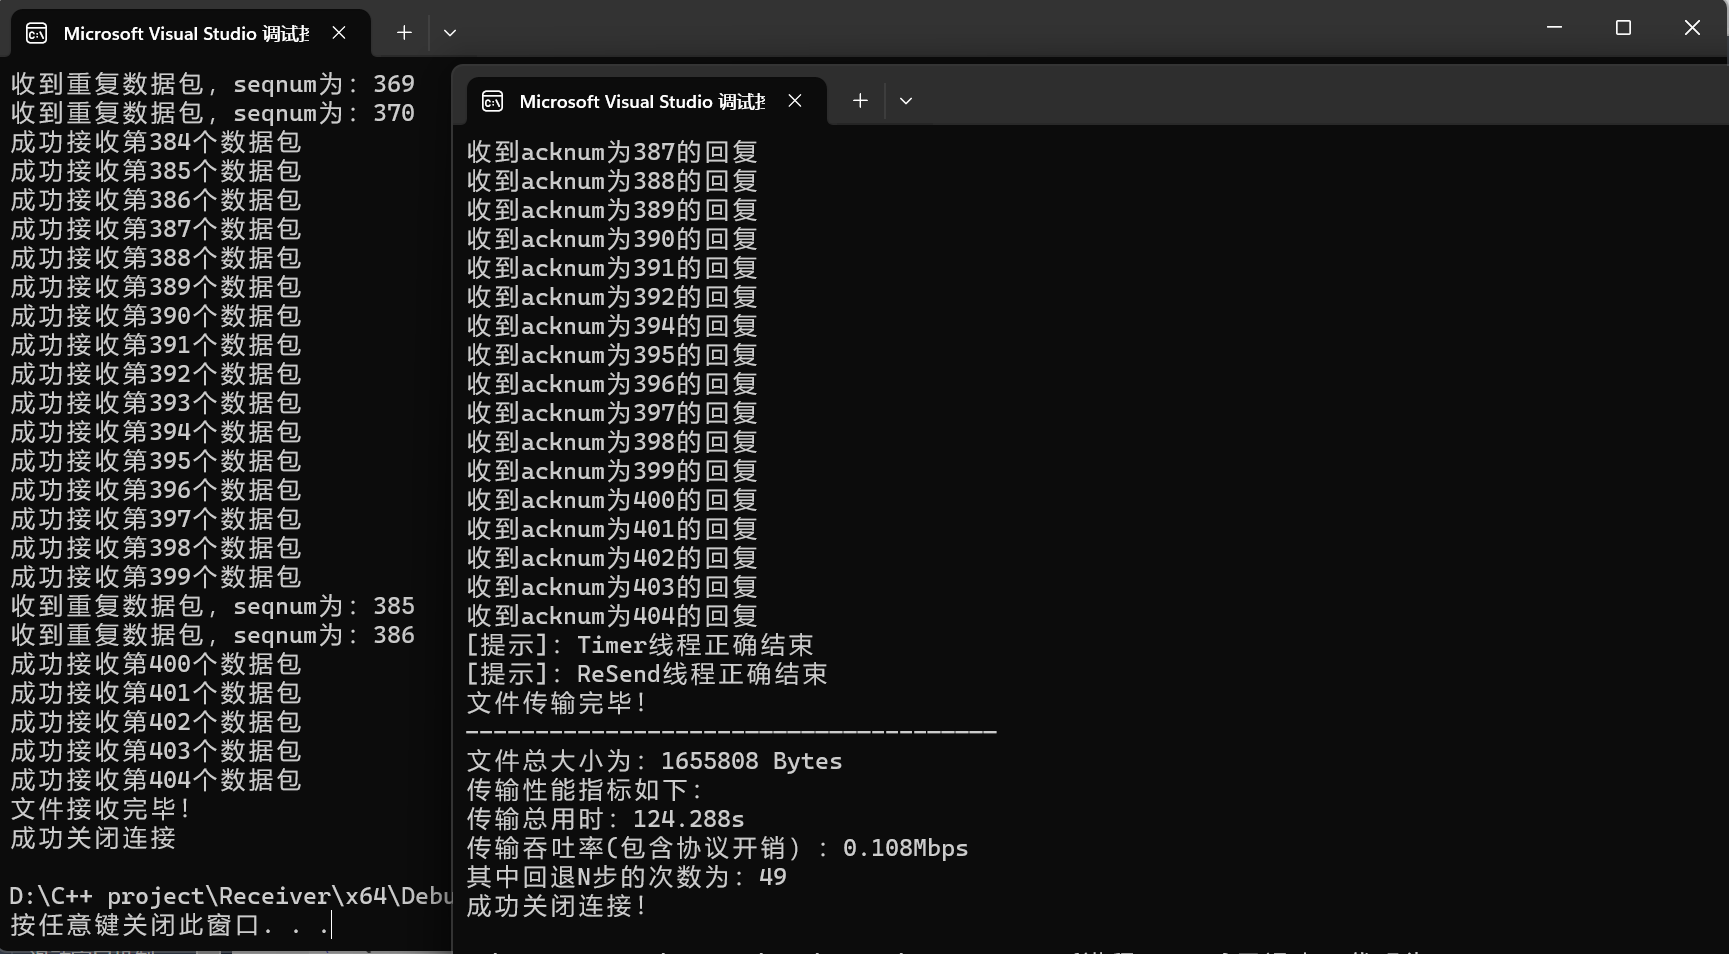
\includegraphics[width=0.8\textwidth]{img/传输helloworld.png}
    \caption{传输helloworld}
\end{figure}
可以看到,程序成功完成了本次传输并且正常关闭连接,在发送端目录下能看到传输的helloworld.txt文件,大小与源文件大小相同。传输1.jpg文件结果如下:
\begin{figure}[H]
    \centering
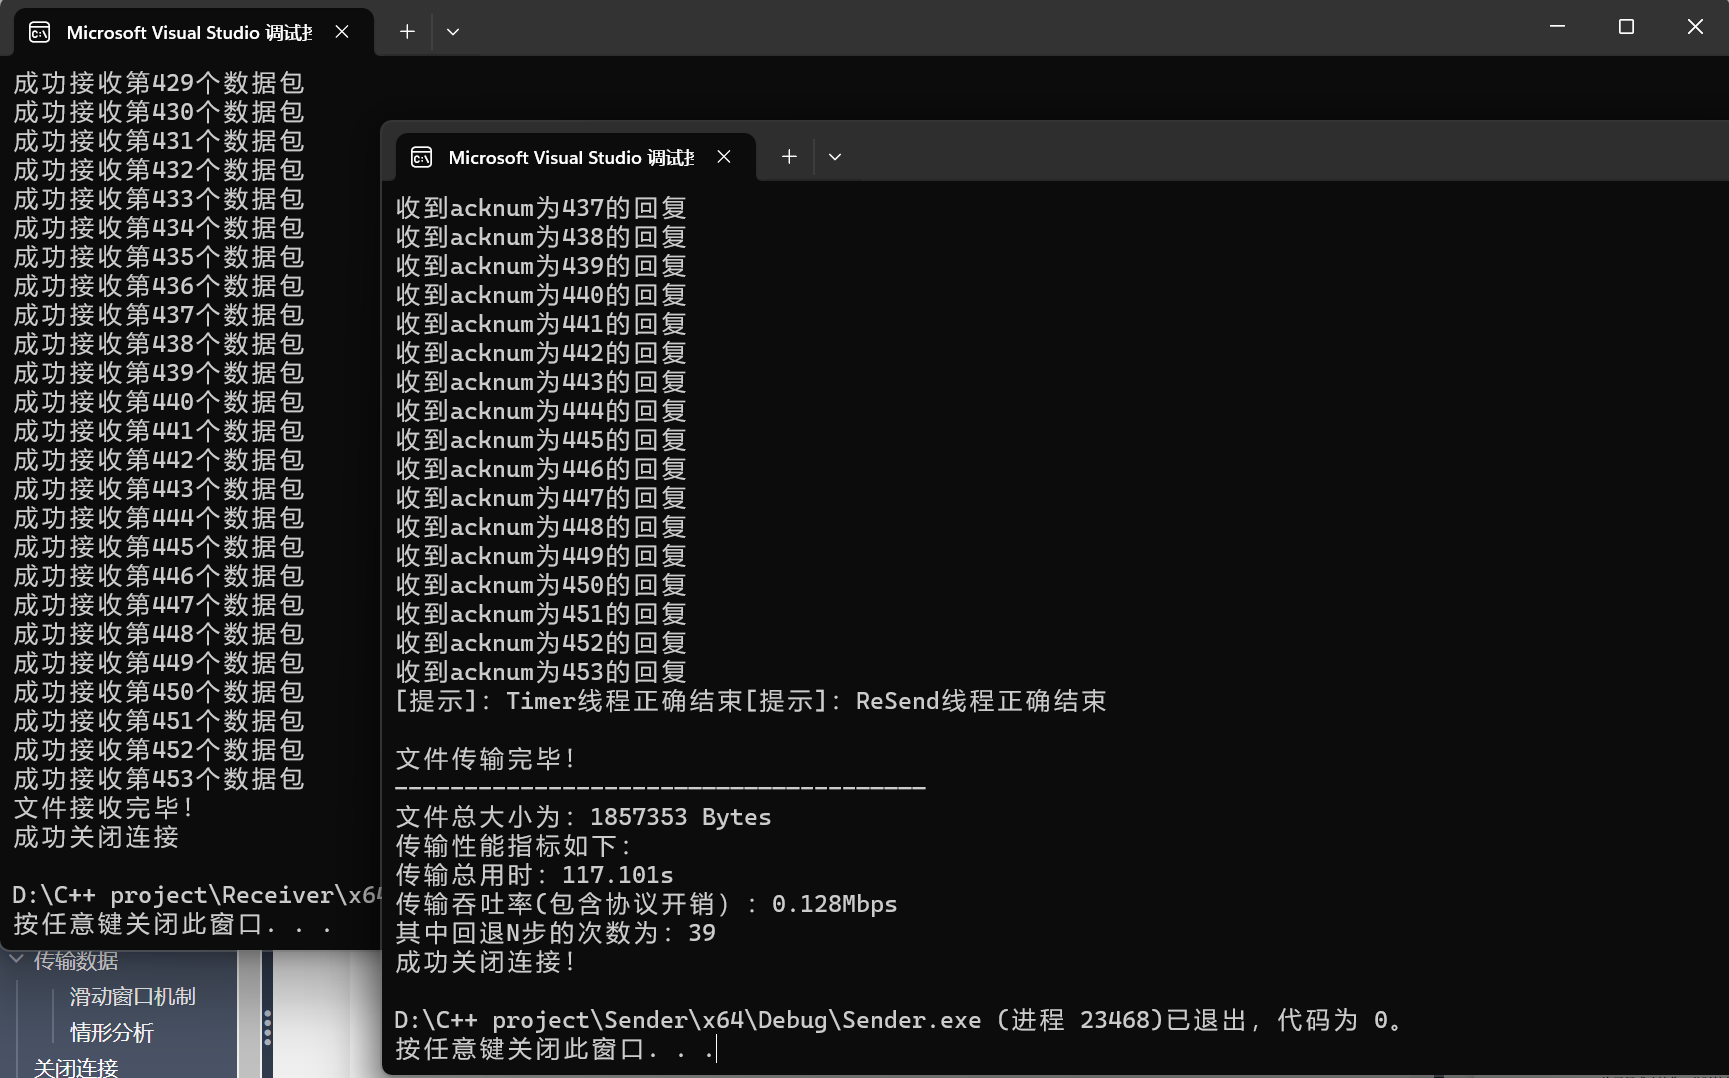
\includegraphics[width=0.8\textwidth]{img/传输图片1.png}
    \caption{传输图片1}
\end{figure}
传输2.jpg文件结果如下:
\begin{figure}[H]
    \centering
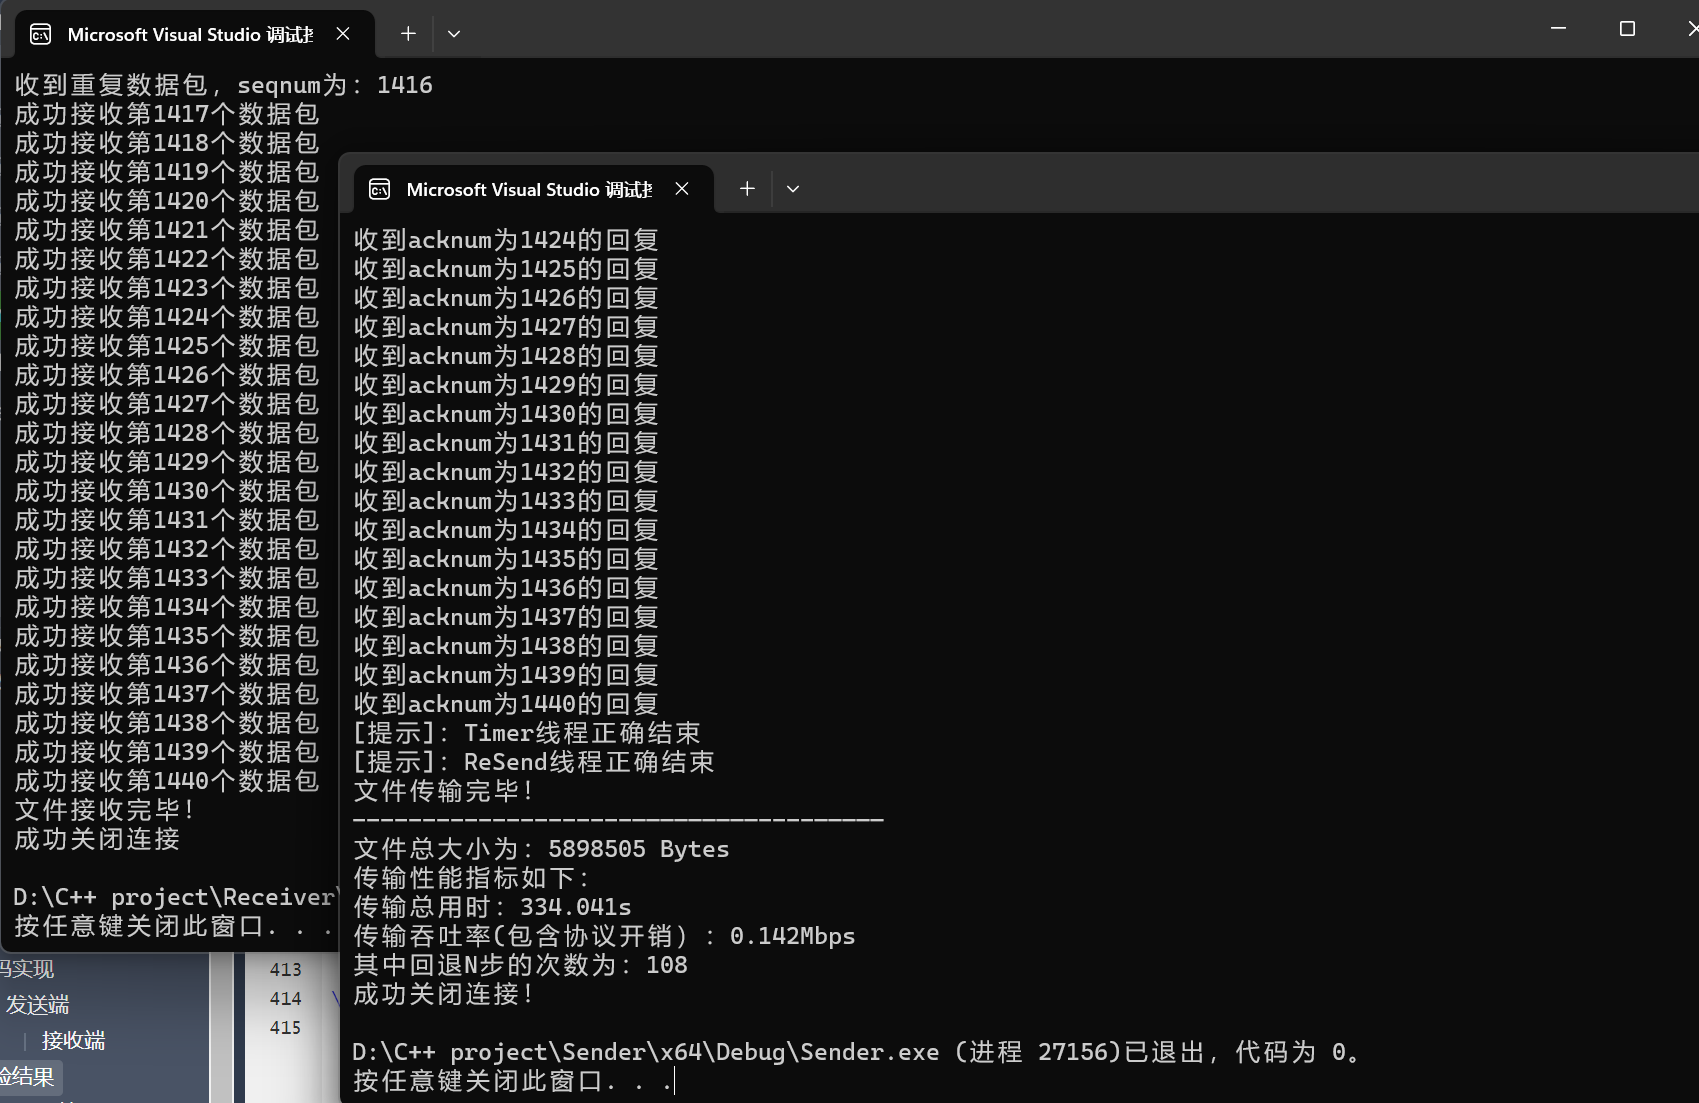
\includegraphics[width=0.8\textwidth]{img/传输图片2.png}
    \caption{传输图片2}
\end{figure}
传输2.jpg文件结果如下:
\begin{figure}[H]
    \centering
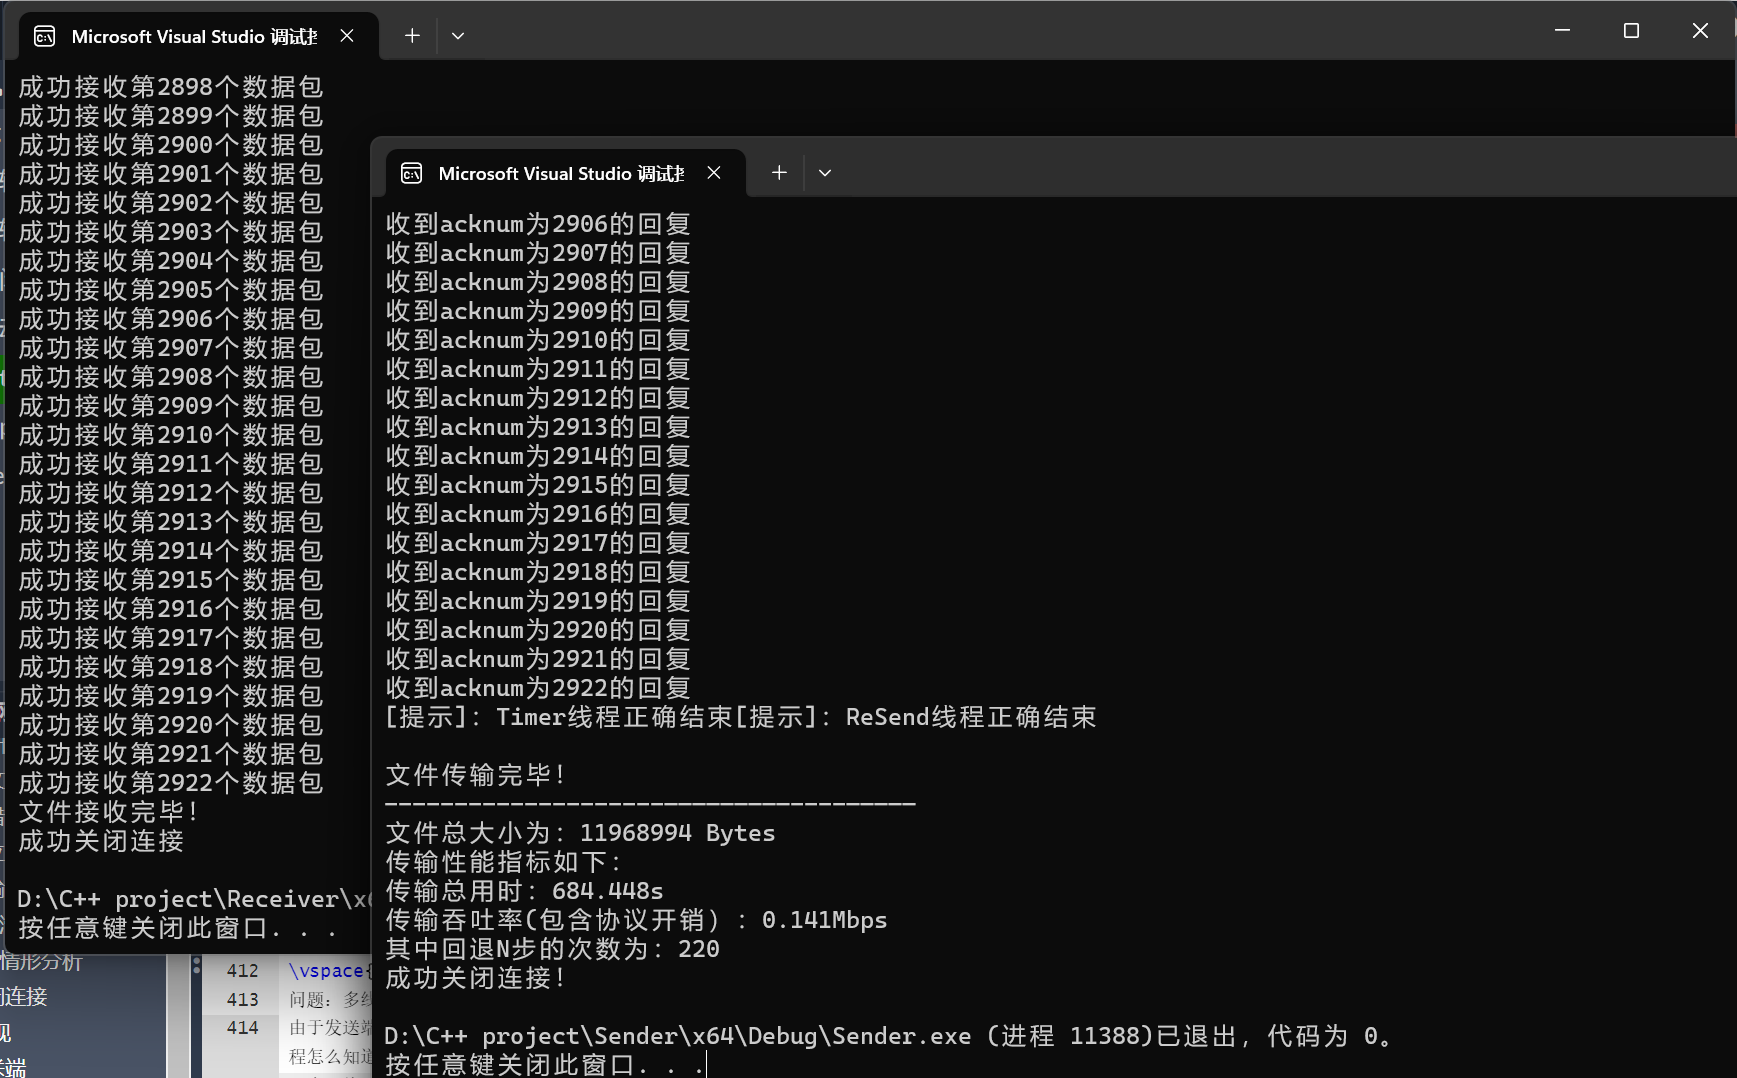
\includegraphics[width=0.8\textwidth]{img/传输图片3.png}
    \caption{传输图片3}
\end{figure}
综上,图片都能够正确传输,且文件大小都与源文件大小相同。同时发现,对于helloworld.txt和1.jpg等较小文件,传输吞吐率波动较大,而对于2.jpg和3.jpg等大文件,可以从图中看到,传输速率基本都为0.14Mbps左右,较为稳定。

\section{遇到的问题\&解决方法}

问题:文件指针不断移动读取原始数据,重传时如何处理?\par
对于这个问题,反复移动文件指针可能出现一系列问题。所以我最开始尝试使用一个队列来保存Base-NextSeq之间的数据包,每次窗口右移的时候队头出队,主线程从原始文件中读取数据,将数据包发送并且放入队尾,同时NextSeq增加。重传的时候,只需遍历整个队列,并发送给接收端即可,从而实现滑动窗口的效果。但由于采用多线程编程,用这种方法的时候程序不时出现运行错误,即窗口的左边界Base已经向前移动,而主线程中的NextSeq即右边界还没来得及向前移动,即队列可能为空后还没来得及入队就要求出队,造成运行错误。\par
后来我选择用一个vector容器来缓存下所有原始数据,窗口的移动依据Base和NextSeq的增加即可,即代码中提到的实现逻辑,不需要出队入队的复杂操作。但缺点是需要缓存下整个文件以及附加的协议开销,空间开销较大。\par

\vspace{1cm}
问题:多线程如何互相通信和交互?\par
由于发送端的逻辑较为复杂,我选择用包含主函数的三个线程来完成发送端的功能,但问题在于线程之间如何相互通信。Resend线程怎么知道什么时候开始重传,Timer线程怎么知道什么时候开始启动计时器。对于该问题,我设置了两个全局变量Flag标志位,两个子线程只需要在while循环中持续监听即可。一旦标志位改变则进行相应操作。但与此同时,另一个问题就是,这部分全局变量属于多线程共享,会进行读写操作,同时读写可能存在风险,所以在程序中我使用了互斥锁来解决这个问题。

\section{思考\&总结}
本次实验用滑动窗口机制来传输数据,在保障可靠传输的前提下实现了流量控制。通过本次实验,我对GBN协议有了更深入的理解。但传输效率上还有很多可以优化的地方,比如接收端和发送端使用同一大小的数据包格式,但单就一端传输一端接收的情形来说,这是不必要的,每次接收端发回ack的时候,4096个字节的数据缓冲区根本没有使用,我会尝试在下一次实验中定义两个不同格式的数据包报文,从而减小在实际传输中的数据开销。
\end{document}
